\documentclass[conference]{IEEEtran}
\usepackage{graphicx,booktabs,amsmath,url,array}
\usepackage[hidelinks]{hyperref}
\graphicspath{{../figures/}}
\newcommand{\pending}{\textit{Planned}}
\begin{document}
\title{Evaluating 30-Day Hospital Readmission Prediction in Patients with Diabetes: Patient-Level Versus Encounter-Level Validation}
\author{\IEEEauthorblockN{Muhammad Shehzore Hashmi}
\IEEEauthorblockA{Electrical and Computer Engineering\\Montana State University\\Bozeman, Montana, USA\\\footnotesize muhammadshehz.hashmi@student.montana.edu}
\and\IEEEauthorblockN{Ahmad Sultan}
\IEEEauthorblockA{Gianforte School of Computing\\Montana State University\\Bozeman, Montana, USA\\\footnotesize ahmad.sultan@student.montana.edu}
\and\IEEEauthorblockN{Akshay Kumar Dosapati}
\IEEEauthorblockA{Gianforte School of Computing\\Montana State University\\Bozeman, Montana, USA\\\footnotesize akshay.dosapati@student.montana.edu}}
\maketitle
\begin{abstract}
Many patients in hospital readmission datasets have more than one encounter, so the way records are split between training and testing can affect reported performance. We study this effect on the Diabetes 130-US Hospitals dataset. After excluding death and hospice discharges, the cohort contains 99,343 encounters from 69,990 patients, of which 11.39\% are readmitted within 30 days. We compare L2 and L1 logistic regression, random forest, and LightGBM under two evaluation designs: a patient-level split, in which no patient appears in both training and test data, and a conventional stratified encounter-level split. Each design is repeated with five predefined seeds, using five-fold cross-validation on the development data and fitting all preprocessing on training folds only. Average precision (AP) is the primary metric. The four weighted models achieve mean patient-level AP between 0.208 and 0.228; LightGBM has the highest mean. Encounter-level test sets contain 41.7\% encounters from patients represented in development data on average. Encounter-level mean AP is modestly higher (+0.005 to +0.013), with a change in model ranking.
 These preliminary results suggest that the choice of split matters more for comparing models than for their overall performance level. Probability calibration, resampling, and subgroup analyses are still in progress.
\end{abstract}
\begin{IEEEkeywords}
readmission, diabetes, grouped validation, repeated encounters, average precision
\end{IEEEkeywords}
\section{Introduction}
Readmission within 30 days increases healthcare costs and can point to problems with recovery, discharge planning, or follow-up care \cite{emi}. Patients with diabetes often have several diagnoses and repeated admissions, which makes their risk hard to assess. A model that flags high-risk encounters at discharge could help hospitals target follow-up resources, but only if its reported performance reflects how it would perform on new patients. We therefore study both the prediction task and how reliably it is evaluated.

The Diabetes 130-US Hospitals dataset contains inpatient encounters recorded between 1999 and 2008 \cite{uci,strack}. Each record is an encounter, not a patient, and many patients have several encounters. If encounters are split at random, the test set will contain both new patients and patients whose other visits were used in training. A patient-level split avoids this by keeping all of a patient's encounters on the same side. Removing the patient ID from the inputs does not solve the problem, because diagnoses, medications, and utilization history often repeat across visits. At the same time, overlap alone does not tell us how much it changes the results; that has to be measured.

Earlier work has studied clinical associations in this dataset \cite{strack}, compared machine learning models \cite{emi}, and adopted patient-level safeguards \cite{afridi}. What is less well documented is how much the choice between patient-level and encounter-level evaluation changes the reported numbers and the ranking of models on the same cohort. We address three research questions. \textbf{RQ1}: How well do four established models rank readmitted encounters when evaluated on unseen patients? \textbf{RQ2}: How do average precision and the model ranking change under encounter-level evaluation, and are the changes consistent across seeds? \textbf{RQ3}: How much patient overlap does encounter-level splitting create, and how do calibration and performance on seen versus unseen patients help interpret the difference? Predictions are made at discharge, and our main target is generalization to unseen patients within this historical dataset.

This report makes three contributions: (1) an audit of the cohort and its repeated patients, which treats unperformed laboratory tests separately from unknown values; (2) a reproducible comparison of four model families under two validation designs and five seeds; and (3) an analysis of patient overlap, model ranking, and calibration that reports uncertainty alongside the point estimates. The target venue is the IEEE Intermountain Engineering, Technology, and Computing Conference.

\section{Related Work}
\subsection{Clinical analysis and predictive benchmarking}
Strack et al. \cite{strack} kept only the first encounter of each patient and excluded death and hospice outcomes. This sidesteps repeated observations by changing the cohort, which suits their analysis of HbA1c testing and readmission. We keep all eligible encounters because the repeated visits are what we want to study, so their sample sizes and associations are not directly comparable to our results.

Emi-Johnson and Nkrumah \cite{emi} compare logistic regression, random forest, XGBoost, and a neural network using a stratified 80/20 split, class weighting, cross-validation, and SHAP. Their methods section does not state that patients were kept apart between training and test data. This does not mean that their results are affected by leakage, only that the reported procedure does not let a reader rule it out. Their study motivates our model comparison, but we focus on how evaluation design changes results rather than on beating published scores.

\subsection{Leakage safeguards and the closest comparison}
Afridi et al. \cite{afridi} describe patient-level partitioning, preprocessing and feature selection within folds, SMOTENC with class weighting, and SHAP/LIME explanations. Their cohort contains 75,081 encounters and they fix the random seed at 42. These safeguards already exist in their work. What we add is a repeated, side-by-side comparison of the two split designs, a measurement of patient overlap, and a check of whether the model ranking is stable across seeds (Table~\ref{tab:literature}).

\begin{table*}[t]
\caption{Comparison of relevant studies and this report. ``Not explicit'' means the published methods do not state it, not that it was done incorrectly.}
\label{tab:literature}\centering\small
\begin{tabular}{>{\raggedright\arraybackslash}p{2.25cm}>{\raggedright\arraybackslash}p{3.25cm}>{\raggedright\arraybackslash}p{3.65cm}>{\raggedright\arraybackslash}p{3.65cm}>{\raggedright\arraybackslash}p{2.65cm}}\toprule
Study & Repeated patients & Validation & Leakage/imbalance handling & Relation to our study\\\midrule
Strack et al. \cite{strack} & First encounter per patient retained & Association modeling; no predictive holdout comparison & Death/hospice exclusions; clinical covariate analysis & Dataset definitions and cohort rationale\\
Emi-Johnson and Nkrumah \cite{emi} & Patient grouping not explicit in split description & Stratified 80/20; five-fold model tuning & Preprocessing pipeline and class weighting reported & Conventional predictive benchmark\\
Afridi et al. \cite{afridi} & Patient groups kept separate & Patient holdout; five-fold grouped validation; seed 42 & Preprocessing, feature selection and SMOTENC within training folds & Closest framework; safeguards already established\\
This report & All eligible encounters retained & Two split designs, five seeds; equal tuning budgets & All fitting on training data; overlap checks; no test resampling & Measures sensitivity to split design and ranking stability\\\bottomrule
\end{tabular}
\end{table*}

\subsection{Validation matched to the intended use}
Saeb et al. \cite{saeb} argue that validation must match how a clinical model will be used: when records from the same person appear in both training and test data, estimates for new patients become overly optimistic. Kapoor and Narayanan \cite{kapoor} place this problem within a broader taxonomy of data leakage in machine learning research. These studies motivate our choice of a patient-level split as the primary evaluation and our explicit overlap measurement. We apply their reasoning to repeated diabetes encounters and keep the encounter-level split as a comparison to measure how much the choice matters. Because the dataset has no usable dates, neither split can test prediction of a known patient's future visits.

\subsection{Imbalance and evaluation}
Precision--recall analysis is more informative than ROC analysis when positives are rare \cite{saito}. We summarize it with non-interpolated average precision rather than the trapezoidal area under the PR curve \cite{apdoc}, and include a constant-score baseline whose AP equals the test prevalence. Scikit-learn's group-aware splitters implement the patient-level design \cite{groupdoc}. Class weighting and resampling both change the meaning of predicted probabilities, so we report Brier scores and an unweighted logistic model alongside ranking metrics. A SMOTENC comparison using imbalanced-learn \cite{imblearn} is planned. LightGBM \cite{lgbm} provides an efficient boosted-tree model alongside random forest and regularized logistic regression.

\section{Data and Preprocessing}
\subsection{Source, cohort, and outcome}
We downloaded the public UCI files \cite{uci}, including the mapping of categorical IDs, and recorded a SHA-256 checksum of the data file. The CSV has 101,766 rows and 50 columns: two identifiers, the outcome, and 47 candidate predictors. Each row is one inpatient encounter. The outcome is $y=1$ for \texttt{<30} and $y=0$ for \texttt{>30} or \texttt{NO}; we did not derive any other readmission labels.

We exclude discharge codes 11, 13, 14, 19, 20, and 21, which denote death or hospice in the supplied mapping. This removes 2,423 rows and leaves 99,343 encounters from 69,990 patients, with 11,314 positives (11.39\%). All age and gender categories are kept. Transfers remain in the cohort, with the discharge category used as a predictor; because a transfer is not an ordinary discharge home, we plan a sensitivity analysis without them.

\subsection{Data quality audit}
The data contain no exact duplicate rows, no repeated encounter IDs, and no rows that become duplicates when the two identifiers are removed. Repeated patients are therefore distinct visits, not duplicated records. In the eligible cohort, 16,341 patients (23.35\%) have more than one encounter, and together they account for 45,694 encounters (46.00\%). The median patient has one encounter, the 99th percentile six, and the maximum 40 (Fig.~\ref{fig:patients}). For this reason we keep repeat visits and group them by patient during evaluation instead of deleting them.

\begin{table}[t]\caption{Audit of the eligible cohort. Unknown values are counted separately from tests that were not performed.}\label{tab:audit}\centering\small
\begin{tabular}{lr}\toprule
Item & Count (percentage)\\\midrule
Eligible encounters / patients & 99,343 / 69,990\\
Positive / negative outcomes & 11,314 / 88,029\\
Patients with repeat encounters & 16,341 (23.35\%)\\
Encounters from repeat patients & 45,694 (46.00\%)\\
Unknown weight & 96,218 (96.85\%)\\
Unknown medical specialty & 48,616 (48.94\%)\\
Unknown payer code & 39,398 (39.66\%)\\
Unknown race & 2,234 (2.25\%)\\
HbA1c not performed & 82,509 (83.05\%)\\
Glucose serum test not performed & 94,191 (94.81\%)\\\bottomrule
\end{tabular}\end{table}
\begin{figure}[t]\centering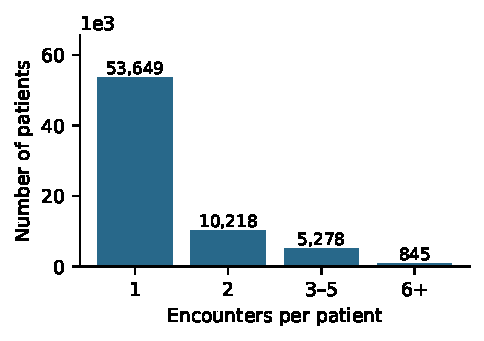
\includegraphics[width=\columnwidth]{patient_counts.pdf}\caption{Eligible patients grouped by number of encounters. Repeat encounters are kept and grouped by patient during the primary evaluation.}\label{fig:patients}\end{figure}

Table~\ref{tab:audit} separates tests that were not performed from values that are unknown. In the HbA1c and glucose fields, \texttt{None} means the test was not performed \cite{strack}, so we read it literally and encode it as a ``Not performed'' category rather than imputing a value. The \texttt{?} marker is encoded as a separate ``Unknown'' category. As planned in Report 1, weight is dropped because 96.85\% of values are missing. The three diagnosis fields have 20, 356, and 1,419 unknown codes, which are also kept as an explicit category. We do not remove outliers or winsorize any variable.

\subsection{Feature representation and leakage prevention}
After dropping weight and the two IDs, 46 input variables remain. The eight count and duration variables are standardized, and all other variables, including age bands and admission and discharge codes, are one-hot encoded. ICD-9 diagnosis codes are grouped into nine clinical categories plus ``Unknown,'' following Strack et al. \cite{strack} but applied to all three diagnosis fields; supplementary E and V codes are assigned to ``Other.'' The scaler and encoder are fitted on training folds only, and categories that appear only in held-out data are ignored. No numerical values are missing in this cohort.

Patient and encounter IDs are used only to form the splits and check them, never as predictors. Fixed cohort rules and code mappings are applied before splitting, and every learned step happens after it (Fig.~\ref{fig:workflow}). We do not build features from other encounters; the prior-visit counts are used as supplied. Because the data lack usable dates and hospital identifiers, our results do not speak to generalization over time or to new hospitals.

\begin{figure*}[t]\centering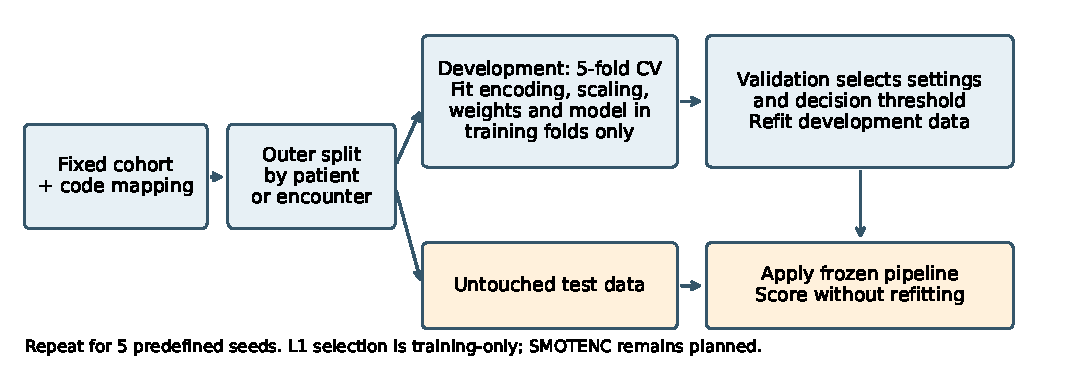
\includegraphics[width=.98\textwidth]{workflow.pdf}\caption{Implemented workflow. The test data are never used for fitting or selection. L1 feature selection happens inside training folds. SMOTENC is planned and will also be restricted to training folds.}\label{fig:workflow}\end{figure*}

\section{Methodology and Implementation}
\subsection{Models}
The simplest baseline is a constant predictor that outputs the readmission rate of the development set. L2-regularized logistic regression is the main model baseline. L1-regularized (LASSO) logistic regression \cite{lasso} drives some coefficients to exactly zero and so performs feature selection within the model. Both use class weights $w_k=n/(2n_k)$ computed from the training labels and minimize a regularized, weighted log loss. The inverse penalty strength $C$ is chosen from $\{0.1,1\}$ for L2 and $\{0.01,0.1\}$ for L1, using the liblinear solver with up to 1,000 iterations. An otherwise identical L2 model without class weights serves as a reference for probability quality.

Random forest \cite{rf} uses 100 trees with maximum depth 12 and square-root feature sampling, with the minimum leaf size chosen from $\{5,20\}$. LightGBM uses 150 boosting rounds, learning rate 0.05, at least 50 samples per leaf, and 15 or 31 leaves. Both use balanced class weights computed from the training data. We deliberately kept each search to two candidates, so that every model receives the same tuning budget and the full study fits in our compute limits; this is not an exhaustive benchmark.

\subsection{Implementation status}
The cohort audit, preprocessing pipeline, all five models, both split designs, repeated tuning and evaluation, and result generation are complete. L1 regularization is the only feature selection method implemented so far; we have not run recursive feature elimination. SMOTENC, probability recalibration, SHAP and permutation importance, and the discharge and subgroup analyses are planned, so the report makes no claims about them.

The experiments use Python 3.12, NumPy, pandas, SciPy, scikit-learn 1.8, LightGBM 4.7, and Matplotlib \cite{numpy,pandas,scipy,sklearn,lgbm,mpl}, running on CPU only; exact versions are stored with the results. We met two practical problems. Random forest was slow on the sparse one-hot matrix, so we pass it a dense 32-bit matrix instead, which gives the same model much faster. A timing pilot also showed that the L1 models were slow at larger $C$ values, so we narrowed the L1 grid before any test results were computed. The five seeds ran in parallel on an eight-core allocation with two threads per model. Each outer partition took 266--367 seconds (median 314), and the longest seed took about 12 minutes for both designs. Code, aggregate results, and the manuscript source are available at\\
\url{https://github.com/Ahmadjajja/Hospital_Readmission_Prediction}.

\section{Experimental Design}
\subsection{Data splitting and model selection}
For each seed in $\{11,23,42,67,101\}$, the patient-level design holds out 20\% of patients (GroupShuffleSplit), together with all of their encounters, so the test set holds about 20\% of encounters. The encounter-level design holds out a stratified random 20\% of encounters. Within the remaining development data, the patient-level design uses StratifiedGroupKFold and the encounter-level design uses StratifiedKFold, each with five folds. The code checks that no patient appears on both sides of any patient-level split.

Each candidate configuration is scored by its mean AP across the five validation folds, and the best one is refitted on the full development set. The decision threshold that maximizes F1 on the out-of-fold development predictions is then fixed and applied to the test set, which is used only once. Both designs use the same candidates and preprocessing, but each selects its own settings, so the comparison measures the effect of the whole evaluation procedure rather than overlap in isolation.

\subsection{Metrics and uncertainty}
Average precision is computed as
\begin{equation}
\mathrm{AP}=\sum_j (R_j-R_{j-1})P_j,
\end{equation}
where $P_j$ and $R_j$ are the precision and recall at the $j$-th threshold of the ranked scores \cite{apdoc}. We also report ROC-AUC, precision, recall, F1, and the Brier score $n^{-1}\sum_i(p_i-y_i)^2$. The threshold affects only precision, recall, and F1. We do not use accuracy, because a model that never predicts readmission would already score about 89\%.

Across seeds we report means and sample standard deviations. The five splits share patients, so their spread shows how much results vary between partitions rather than providing a formal confidence interval. To compare models on the same patients, we use the seed-42 patient-level test set, chosen in advance, and draw 1,000 bootstrap samples of patients (resampling seed 2026). All encounters of a sampled patient are included together, and every model is evaluated on the same samples, giving paired percentile 95\% intervals for the AP difference from L2. These intervals hold the fitted models fixed and are not adjusted for multiple comparisons. We do not compute paired intervals between the two designs, because their test sets differ.

\subsection{Overlap analysis and success criteria}
For each encounter-level test set, we record the share of test encounters whose patient also appears in the development data, and we report results separately for seen and unseen patients. We consider the study successful if it produces a complete, reproducible comparison with uncertainty estimates, even if the more complex models do not beat the baseline or the gap between designs turns out to be small.

\section{Implementation Progress and Initial Findings}
\subsection{Completed experiments and performance}

All ten outer partitions completed: 500 candidate fits, 50 selected model fits, and ten constant-reference evaluations. The exported metrics contain 60 evaluated model/protocol/seed combinations. Automated checks recompute metrics from predictions, verify labels against source records, and verify partition integrity. No convergence warnings were observed in the completed-run logs. Table~\ref{tab:performance} and Fig.~\ref{fig:comparison} summarize the main results. Values are preliminary benchmark findings, not clinical validation.

\begin{table}[t]\caption{Test performance, mean $\pm$ sample SD across five seeds. Constant AP equals each test set\textquotesingle s positive fraction.}\label{tab:performance}\centering\footnotesize\begin{tabular}{llcc}\toprule Model & Split & AP & ROC-AUC\\\midrule

L2 logistic & Patient & 0.216 $\pm$ 0.006 & 0.663 $\pm$ 0.003 \\

L2 logistic & Encounter & 0.221 $\pm$ 0.002 & 0.669 $\pm$ 0.005 \\

L1 logistic & Patient & 0.215 $\pm$ 0.006 & 0.665 $\pm$ 0.003 \\

L1 logistic & Encounter & 0.222 $\pm$ 0.002 & 0.671 $\pm$ 0.004 \\

Random forest & Patient & 0.208 $\pm$ 0.002 & 0.665 $\pm$ 0.005 \\

Random forest & Encounter & 0.221 $\pm$ 0.002 & 0.673 $\pm$ 0.004 \\

LightGBM & Patient & 0.228 $\pm$ 0.006 & 0.673 $\pm$ 0.002 \\

LightGBM & Encounter & 0.238 $\pm$ 0.004 & 0.679 $\pm$ 0.003 \\

L2 unweighted & Patient & 0.216 $\pm$ 0.006 & 0.662 $\pm$ 0.003 \\

L2 unweighted & Encounter & 0.221 $\pm$ 0.002 & 0.668 $\pm$ 0.005 \\

Constant & Patient & 0.112 $\pm$ 0.002 & 0.500 $\pm$ 0.000 \\

Constant & Encounter & 0.114 $\pm$ 0.000 & 0.500 $\pm$ 0.000 \\

\bottomrule\end{tabular}\end{table}

\begin{figure}[t]\centering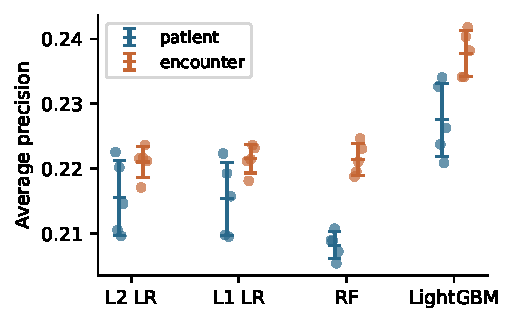
\includegraphics[width=\columnwidth]{comparison.pdf}\caption{AP across five seeds. Points are individual runs; marks and error bars show means and sample standard deviations.}\label{fig:comparison}\end{figure}

LightGBM has the highest mean patient-level AP (0.228), compared with 0.216 for weighted L2 and 0.112 for the constant reference. The encounter-minus-patient differences in mean AP are +0.0055 (L2 logistic), +0.0062 (L1 logistic), +0.0132 (Random forest), +0.0102 (LightGBM). These are descriptive differences across separately constructed test sets. They are not paired causal effects of overlap.

\subsection{Overlap and conditional uncertainty}

Patient-level holdouts have zero patient overlap by assertion. Encounter-level overlap ranges from 41.34\% to 42.10\% of test encounters (mean 41.70\%). Patient-arm test prevalence ranges from 10.99\% to 11.41\%; the corresponding test sizes range from 19,717 to 19,991. The constant-reference results make this variation explicit.

For LightGBM within encounter-level holdouts, mean AP is 0.279 for seen patients and 0.157 for unseen patients. Their mean positive fractions are 20.10\% and 5.16\%, respectively. The case-mix and prevalence difference prevents interpreting this subset contrast as an isolated overlap effect.

For the prespecified patient holdout at seed 42, paired AP differences relative to weighted L2 and their 95\% patient-bootstrap intervals are L1 logistic: -0.0010 [-0.0026, +0.0006]; Random forest: -0.0095 [-0.0169, -0.0021]; LightGBM: +0.0138 [+0.0073, +0.0214]. These conditional, unadjusted intervals complement rather than replace the repeated-seed summaries.

\subsection{Thresholds and probability quality}

\begin{table}[t]\caption{Patient-level threshold and probability diagnostics: means across five runs. Thresholds maximize development out-of-fold F1.}\label{tab:diagnostics}\centering\footnotesize\begin{tabular}{lrrrr}\toprule Model & Precision & Recall & F1 & Brier\\\midrule

L2 logistic & 0.193 & 0.475 & 0.274 & 0.225\\

L1 logistic & 0.193 & 0.476 & 0.275 & 0.225\\

Random forest & 0.189 & 0.500 & 0.274 & 0.219\\

LightGBM & 0.211 & 0.435 & 0.284 & 0.215\\

L2 unweighted & 0.197 & 0.447 & 0.272 & 0.095\\

Constant & 0.000 & 0.000 & 0.000 & 0.099\\

\bottomrule\end{tabular}\end{table}

Table~\ref{tab:diagnostics} reports the precision--recall trade-off after development-only threshold selection. Unweighted L2 has mean Brier score 0.095, compared with 0.225 for weighted L2. The calibration diagnostic (Fig.~\ref{fig:calibration}) illustrates why class-weighted scores should not automatically be interpreted as calibrated risks. Brier score combines discrimination and calibration; a lower value alone does not establish perfect calibration. No probability correction has yet been fitted.

\begin{figure}[t]\centering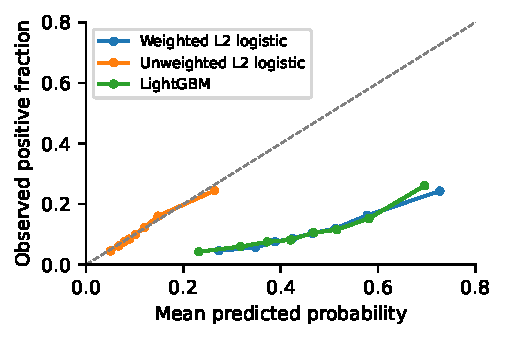
\includegraphics[width=\columnwidth]{calibration.pdf}\caption{Calibration diagnostic for the prespecified patient holdout, seed 42. Eight quantile bins; dashed line indicates ideal calibration. This is a diagnostic, not a fitted correction.}\label{fig:calibration}\end{figure}


\section{Discussion, Limitations, and Responsible Use}
The two designs answer different questions. A patient-level split estimates performance on new patients, while an encounter-level split mixes new and returning patients. Our results show that the encounter-level design gives only slightly higher scores, but the gain is uneven across models and is enough to change which model looks best. Because the two designs use different test sets, the gap cannot be attributed to overlap alone.

Our cohort differs from those of earlier studies, mainly because we keep repeat encounters and transfers, so comparing our scores directly with published numbers would be misleading. The small tuning grids may favor some models over others. Encounter-level metrics also give more weight to frequent patients; we plan a patient-weighted analysis to check this. Readmissions to hospitals outside the network are not recorded, and clinical practice and coding have changed since 1999--2008.

The dataset is released under CC BY 4.0 \cite{uci}. It is deidentified, but demographic fields remain sensitive, and we make no attempt at reidentification. Race, gender, and age groups may be unevenly represented or recorded, and we have not yet analyzed performance by subgroup, so we make no fairness claims. The models are research benchmarks, not clinical tools, and any feature importance we report later will describe associations, not causes.

\section{Response to Feedback and Updated Outline}
We addressed each comment on Progress Report 1 as follows.
\begin{itemize}
\item \textit{Figure size and readability:} the workflow figure (Fig.~1 in Report 1) is now Fig.~\ref{fig:workflow}, redrawn at full page width with larger labels.
\item \textit{Order of splitting, feature selection, and resampling:} the new figure shows the split first. Preprocessing and L1 feature selection are fitted only within training folds, and planned resampling will be restricted to training folds as well.
\item \textit{Repeated seeds:} every comparison is repeated with five predefined seeds, and we report means, standard deviations, and individual runs (Table~\ref{tab:performance}, Fig.~\ref{fig:comparison}).
\item \textit{Literature and Afridi et al.:} Table~\ref{tab:literature} compares how prior studies handle repeated patients, validation, and leakage. Section~II-B explains what our study adds beyond Afridi et al.
\item \textit{Duplicates, missing data, status, and references:} Section~III-B reports the duplicate checks and the encounters-per-patient distribution, and Table~\ref{tab:audit} separates unperformed tests from unknown values. Completed and planned work are labeled throughout, and all references follow IEEE style.
\end{itemize}
The research questions, dataset, and models are unchanged; we added an unweighted logistic model to study calibration. Table~\ref{tab:outline} gives the updated outline.

\begin{table}[t]\caption{Updated outline of the final paper.}\label{tab:outline}\centering\footnotesize
\begin{tabular}{>{\raggedright\arraybackslash}p{1.65cm}>{\raggedright\arraybackslash}p{5.8cm}}\toprule
Section & Content, evidence, and planned outputs\\\midrule
Abstract & Update findings after the remaining analyses.\\
Introduction & Keep RQs and contributions; adjust scope to the final evidence.\\
Related work & Add calibration and resampling literature; extend Table I.\\
Data & Keep the audit table and encounter-frequency figure.\\
Methods & Add SMOTENC and calibration settings.\\
Experiments & Same seeds and grouping; add sensitivity and subgroup protocols.\\
Results & Current AP/ROC tables plus an imbalance table, a subgroup table, and a feature-importance figure.\\
Discussion & Interpret ranking changes, uncertainty, and calibration across designs.\\
Limitations & Historical data, repeated patients, no dates, representation, external validity.\\
Conclusion & Answer each RQ with the completed evidence.\\\bottomrule
\end{tabular}\end{table}

\section{Remaining Work and Responsibilities}
Table~\ref{tab:plan} lists the work remaining before Progress Report 3. Ahmad Sultan leads implementation and reproducibility, Muhammad Shehzore Hashmi leads validation and statistical checks, and Akshay Kumar Dosapati leads the literature review and figures. All three members review the code, the cited papers, the results, and the manuscript. The project is on the schedule proposed in Report 1: the primary evaluation was planned for early November, and the imbalance, calibration, and sensitivity analyses for mid-November. The scope has not changed. If time runs short, we will run resampling on one model only and report subgroup counts without comparisons where groups are too small.

\begin{table}[t]\caption{Remaining work toward Progress Report 3, in priority order.}\label{tab:plan}\centering\footnotesize
\begin{tabular}{p{1.05cm}p{4.2cm}p{2.15cm}}\toprule
Target & Task and dependency & Lead\\\midrule
Week 1 & Review literature on patient- versus record-level validation and calibration; extend Table I & Shehzore, all\\
Week 1--2 & SMOTENC within training folds on a limited model set; needs a mixed-type pipeline & Ahmad\\
Week 2 & Recalibration fitted on development data; transfer and patient-weighted sensitivity analyses & Ahmad, Shehzore\\
Week 2--3 & Subgroup counts and errors; feature-importance figure; needs enough positives per group & Akshay, all\\
Before R3 & Add imbalance and subgroup tables and calibration and importance figures; final review & All members\\\bottomrule
\end{tabular}\end{table}

\section{Preliminary Conclusion}
Repeated patients account for nearly half of all encounters. Evaluating on encounters instead of patients raises AP only slightly but changes how the models compare. LightGBM performs best on unseen patients, and the class-weighted models need recalibration before their outputs can be read as risks.

\bibliographystyle{IEEEtran}
\bibliography{references}
\end{document}
